\documentclass{sciposter}

\usepackage{epsfig}
\usepackage{amsmath}
\usepackage{amssymb}
\usepackage{multicol}
\usepackage{graphicx}
\usepackage{color}
\usepackage[english]{babel}
\usepackage[T1]{fontenc}
\usepackage[ansinew]{inputenc}

\hyphenation{ce-llu-lo-se}

\def\T{{ \mathrm{\scriptscriptstyle T} }}

\definecolor{BoxCol}{rgb}{0.87,0.9,1}
\definecolor{SectionCol}{rgb}{0,0,0.5}
\definecolor{titlecolor}{rgb}{0,0,0.5}
\definecolor{remarkcolor}{rgb}{0,0,0.5}

\title{\textcolor{titlecolor}{Poster title}}

%\vspace{5cm}

\author{Fulanito de tal 1\\
         Fulanito de tal 2\\
         Fulanito de tal 3}

\institute{Universidad Nacional de Colombia\\
			Universidad Pontificia Bolivariana\\
			Universidad del Norte}

\email{yreod@unal.edu.co, wusjf@udea.edu.co, dyuej@uninorte.edu.co}

\leftlogo[1.5]{unal.png}  % defines logo to left of title (with scale factor)
\rightlogo[1.5]{upb.png}  % same but on right

\vspace{1.5cm}
%!-------------------------------------------------------------------------------
\begin{document}

\begin{boldmath}

\maketitle

%%% Begin of Multicols-Enviroment
\begin{multicols}{3}

%!-------------------------------------------------------------------------------
\begin{abstract}
Clustered data are, nowadays, available in multiple disciplines. Statistical modeling of these data is usually performed using Generalized Linear Mixed Models (GLMMs), proposed by Breslow \& Clayton (1993), to account for the  hierarchical structure in the data. One problem of interest is to determine whether, in the fitted model, the variance component ($\sigma^2$) of the random effects is statistically zero (that is, the random effect does not explain much of the variance and should be excluded from the model). In the literature, this feature is assessed using a variance component test. Here we present the results of a statistical simulation study assessing the performance of two variance component tests in the context of GLMMs, when a binary and Gamma response variables are considered. In particular, the likelihood ratio (LR) and the permutation tests are evaluated, and the impact of misspecifying the true distribution of the random effects is measured as a function of the number of individuals per cluster and the true value of $\sigma^2$.
\end{abstract}
%\vspace{0.5cm}
%!-------------------------------------------------------------------------------
\section{Introduction}
Clustered data are commonly collected in studies on medical, social, and behavioral sciences. This type of data arise when there is a hierarchical or clustered structure in the data such as individuals nested in institutions or organizations (i.e., students in schools, employees in firms, or patients in hospitals). Mixed models, hierarchical models or multilevel regression models provide an attractive framework to accommodate the overdispersion and dependence of this type of data (Zhu \& Zhang, 2006). Many of the models used in these fields fall under the frame of Generalized Linear Mixed Models (GLMMs). A fundamental question in this models is about the heterogeneity among clusters, which is equivalent to test whether $\sigma^2$, the variance component associated to the random effects, is statistically zero. This test is known as a \textit{variance component test}, and can be approached using the likelihood ratio (LR) and permutation tests (LRs), and have important implications in statistical modeling of clustered data. Here we use a statistical simulation approach to determine, which of the aforementioned tests is more appropriate to determine whether $\sigma^2$ is effectively zero. To do this, different statistical distributions and several prespecified values of $\sigma^2$ are utilized to generate the vector of random effects, followed by the underlying data to be modeled. 
%\vspace{0.5cm}
%!-------------------------------------------------------------------------------
\section{GLMMs}
GLMMs, proposed by Breslow \& Clayton (1993), have been extensively in many applications where clustered and/or longitudinal data are available. Let $y_{ij}$ the $j$th response variable within the $i$th cluster $(i=1,2,\ldots,m; j=1,2,\ldots,n_i)$. In a GLMMs with random intercept, it is assumed that, conditional to the random effects $b_i$, the outcome $y_{ij}$ is  independent with the following structure:
\begin{align} \label{glmm_est}
\begin{split}
y_{ij} \mid b_i &\sim \text{independent in } F_y,  \\
g(\mu_{ij}) &= \boldsymbol{X}_{ij} \boldsymbol{\beta} + b_i ,  \\ 
b_i &\overset{ind}{\sim} N(0,\sigma^2), 
\end{split}
\end{align}
where $F_y$ belongs to the exponential family, $g(\cdot)$ is a known link function, $\boldsymbol{X}_{ij}$ is the vector of covariates for the $j$th observation in the $i$ cluster, and $\boldsymbol{\beta}$ is the parameter vector for the fixed effects.

%!-------------------------------------------------------------------------------
\section{Variance component test}
Among the tests available in the literature for testing 
\begin{equation}\label{H0}
H_0:\sigma^2=0 \text{ vs. } H_A:\sigma^2>0, 
\end{equation}
where $\sigma^2$ is the variance of random intercept, the LR test is the most commonly used test because of its theoretical properties and straightforward construction. In a GLMM with random intercept, we are interested in testing $H_0$ in (\ref{H0}) using a type I error probability $\alpha$. The statistic for the LR test is calculated as 
\begin{equation} \label{T}
T=-2\log \left( \frac{L_0}{L_A} \right)
\end{equation}
where $L_0$ and $L_A$ are the likelihood model under $H_0$ and $H_A$, respectively. Under $H_0$, the asymptotic null distribution of $T$ is a GLMM with random intercept is a 50:50 mixture between a $\chi_0^2$ and $\chi_1^2$ distributions (Zhang \& Lin, 2008).\\

The permutation test (PT) is a modification of LR test proposed by Fitzmaurice \& Lipsitz (2007). The idea behind the PT is that, when $H_0$ in (\ref{H0}) is true, the heterogeneity between clusters is non-existing. This result implies that we could mix the clusters without changing the decision. In what follows we present the implementation of the PT given by Fitzmaurice \& Lipsitz (2007).\\ 

\begin{enumerate}
	\item Calculate the LR test statistic in the original sample and denote it by $T_{obs}$.
	\item Permute the cluster indexes while holding fixed the number of units within a cluster, $n_i$, and calculate the LR test statistic $T$.
	\item Repeat step 2, $k$ times, to obtain $T_1,T_2,\ldots,T_k$, where $T_k$ is the LR statistic in (\ref{T}) for the $k$th permutation of the original clusters.
	\item Determine the PT  $p$-value as the proportion of permutation samples where $T_i\geq T_{obs}$ for $i=1,2,\ldots,k$.
\end{enumerate}

%!-------------------------------------------------------------------------------
\section{Simulation study}

In order to compare the two variance component tests, we consider a GLMM with random intercept and a response variable following a binary distribution. In both cases, the random intercept was sampled from four true statistical distributions (Normal, Log-Normal, Exponential and Uniform). For the fitting procedure, normality of the random intercept was assumed. The model considered in this case can be summarised as follows:
\begin{equation} \label{binary_model}
\text{logit} \{ P(y_{ij} = 1 \mid b_i) \} = \beta_0 + \beta_{b} x_1 + \beta_{w} x_2 + b_i,
\end{equation}
where $i=1,2,\ldots,m$ represents the cluster and $j=1,2,\ldots,n_i$ represents the number of observations per cluster. The between-cluster covariate $x_1 \sim \text{Poisson}(\lambda=2)$ and $x_2$ is a within-cluster covariate following a $U(0, 1)$ distribution. The true model parameters are $\beta_0=-2.5$, $\beta_{b}=2$ and $\beta_{w}=1$.\\

The random effects $b_i$ in model (\ref{binary_model}) were generated from normal, uniform, exponential and log-normal distributions. For exponential and log-normal case, the random values were transformed to ensure the zero mean and variance $\sigma^2$. In the next figure we show the distributions used to generate the random intercepts for the case $\sigma^2=1$.

\begin{figure}[h]\centering
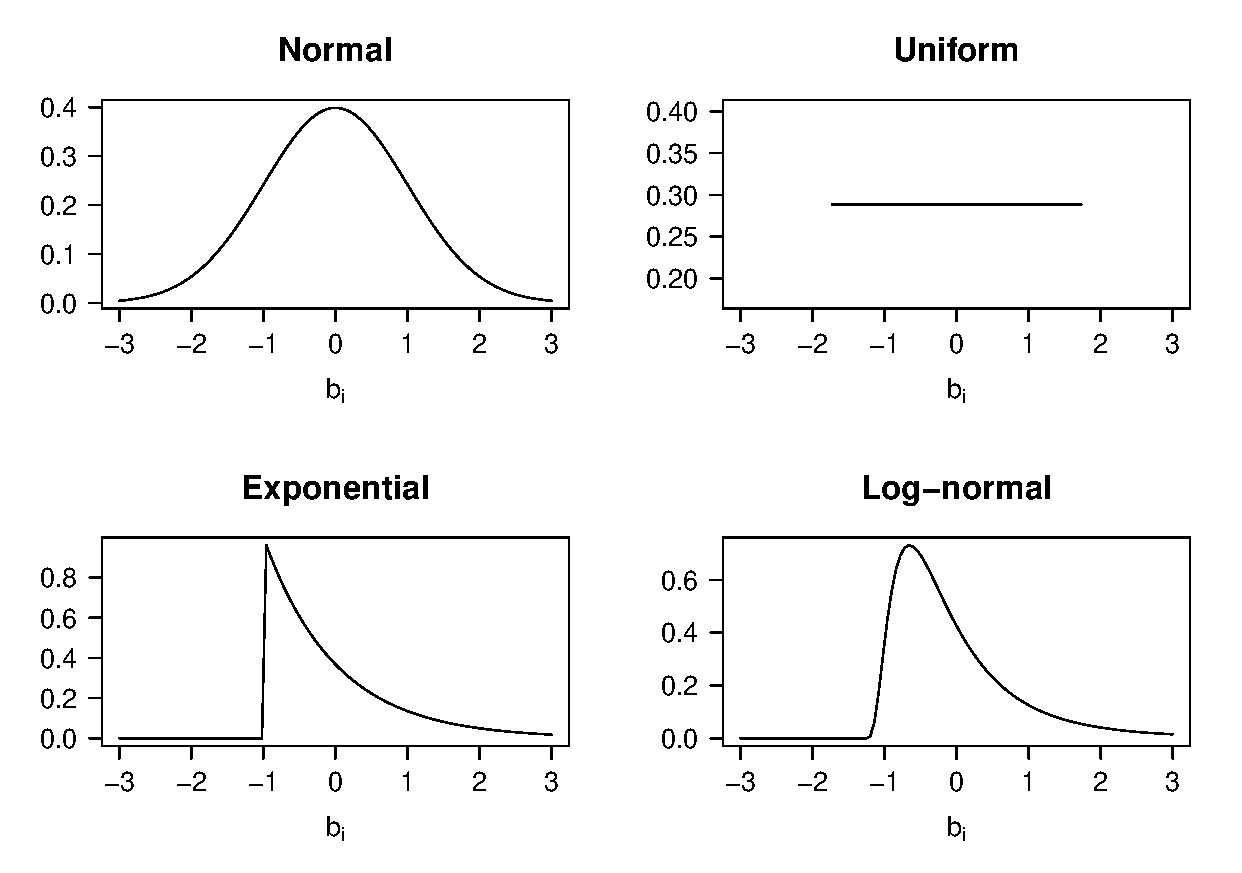
\includegraphics[scale=1.05]{REdist.pdf}
\caption{\label{REdist} Distributions for the random effect considered to generate $b_i$. In this figure the mean of random effects was zero with $\sigma^2=1$.}
\end{figure}
%\vspace{7cm}
%!-------------------------------------------------------------------------------
\section{Results}
Figure \ref{results} displays the main results for the binary GLMM outlined in expression (\ref{binary_model}). Overall, the average rejection rate (ARR) of $H_0$ in (\ref{H0}) of the LR test and the PT are affected for the number of individuals per cluster (parameter $n_i$ in our simulation approach) and the pre-specified value of $\sigma^2$, but have a similar behaviour regardless of the true distribution of the random effects. To directly compare the ARRs between the LR test and PT, the ratio
\begin{equation}
\gamma=\frac{\text{ARR}_{\text{LR}}}{\text{ARR}_{\text{PT}}}
\end{equation}
was calculated.  Here, values of $\gamma>1$ indicate that the LR test outperforms the PT; values of $\gamma<1$ indicate that the LR test outperforms the PT, and $\gamma=1$ indicate that the LR test and PT produce equivalent rejection rates. When the number of individuals per cluster is small (that is, $n_i<5$), the PT has a higher ARR than the LR test (see third column in Figure \ref{results}). Our results show that the LR test and PT are not significantly affected by any of the aforementioned parameters, but that the PT outperforms the LR test. This result has important implications when modelling clustered and/or longitudinal data.

\begin{figure}[htb]
  \centering
  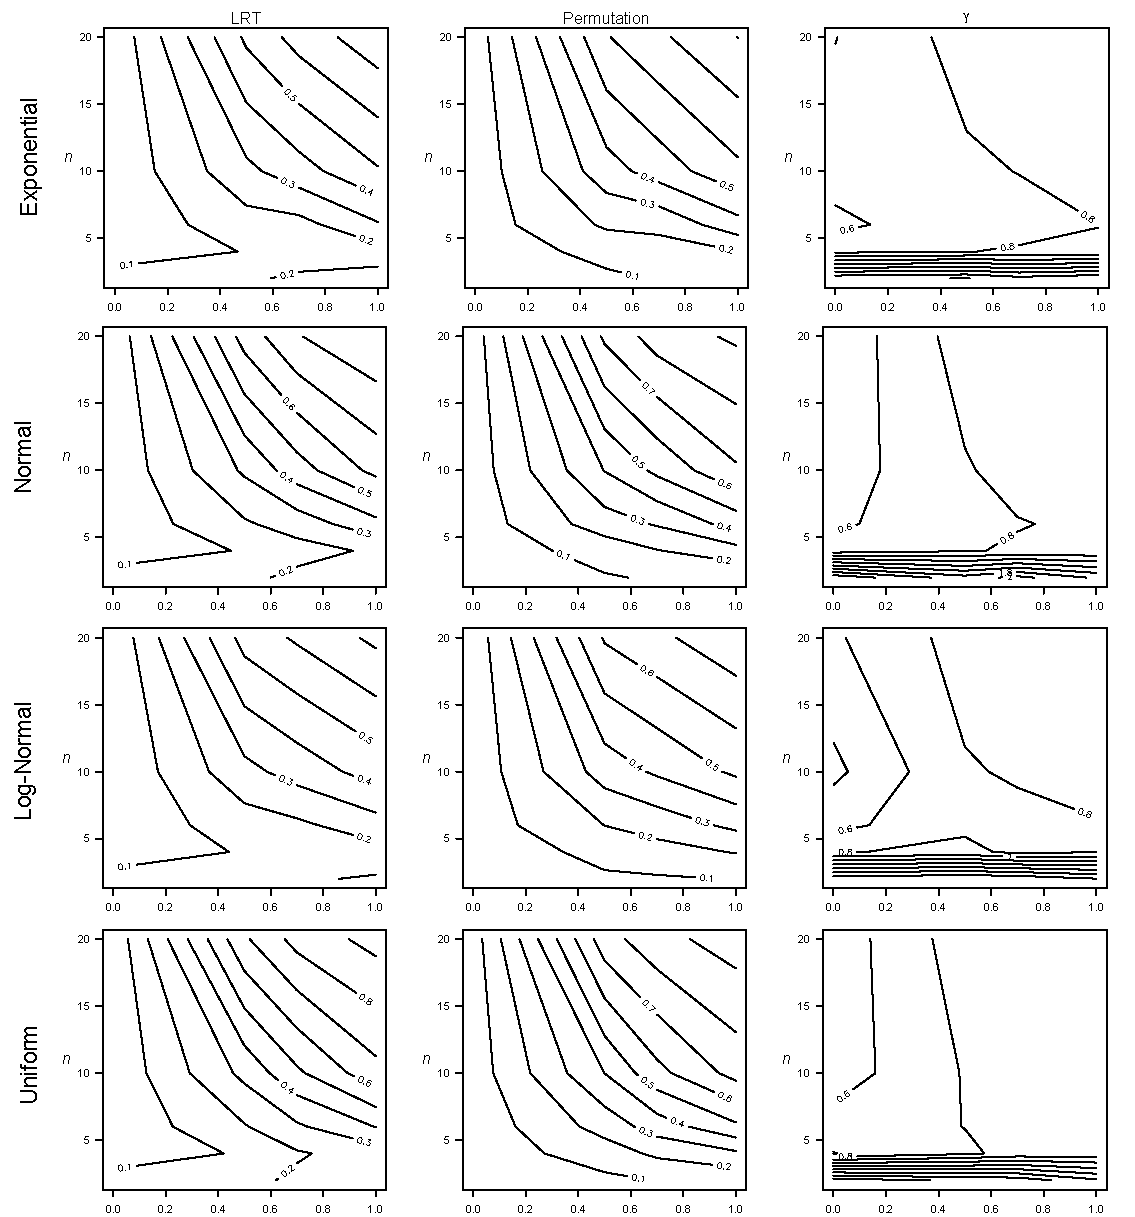
\includegraphics[scale=1.24]{resbinary.pdf}
  \caption{ARR of $H_0:\sigma^2=0$ in (\ref{H0}) in the binary GLMM as  a function of $n_i$ and $\sigma^2$ for each distribution of the random effects.  The third column corresponds to $\gamma$.}\label{results}
\end{figure}
%!-------------------------------------------------------------------------------
\section{Conclusions}
We found that LR and permutation tests have similar ARR patterns regardless the change in the true random effect distribution. We found that ARR increases as $n$ and/or $\sigma^2$ increase.

%!-------------------------------------------------------------------------------
\section*{References}
\begin{description}
\item[Breslow, N.E. and Clayton, D.G.] (1993).
     Approximate inference in ge\-ne\-ra\-li\-zed linear mixed models.
     {\it Journal of the American Statistical Association}, {\bf 88},
     9\,--\,25.
     
\item[Fitzmaurice, G.M. and Lipsitz, S.R.] (2007).
     A Note on Permutation Tests for Variance Components in Multilevel Generalized Linear Mixed Models.
     {\it Biometrics}, {\bf 63},
      942\,--\,946.
     
\item[Zhang, D. and Lin, X.] (2008).
     {\it Variance Component Testing in Generalized Linear Mixed Models for Longitudinal/Clustered Data and other Related Topics} in Dubson, D.B. (2008) Random Effect and Latent Variable Model Selection.
     New York: Springer.
\end{description}


%!-------------------------------------------------------------------------------
\end{multicols}
\end{boldmath}
\end{document}
%!-------------------------------------------------------------------------------
